\documentclass[11pt, fleqn, xcolor=x11names]{beamer}
\usetheme{myamsterdam} %тема\
\usecolortheme{default}
\usepackage[utf8x]{inputenc}
\usepackage[english,russian]{babel}
\usepackage[T2A]{fontenc}
\usepackage{amsmath}
\usepackage{amsfonts}
\usepackage{amssymb}
\usepackage{hyperref}
\usepackage{graphics, graphicx}
\usepackage{color}
\usepackage{hyperref}
\usepackage{enumerate}
\usepackage{amsmath}
\usepackage{amsfonts}
\usepackage{amssymb}
\usepackage{csvsimple}
\usepackage{tikz}
\usepackage{pgfplots}
\usepackage{cmap}
\usepackage{fancyvrb}
\usepackage{caption}
\usepackage{bm}

\usepackage{codestyle}
\usepackage[outputdir=out,cache=false]{minted}
\usemintedstyle{default}


\usepackage{tikz}
\usetikzlibrary{arrows,positioning}
\usepackage{listings}
\lstset{language=Python}

\setbeamertemplate{navigation symbols}{} % отключить навигационные значки
\setbeamertemplate{footline}{%
    \hspace{0.94\paperwidth}%
    \usebeamerfont{title in head/foot}%
    \insertframenumber\,/\,\inserttotalframenumber%
} % переопределить нижнуюю панель, убрать всё кроме номера слайда


%\usefonttheme[onlylarge]{structurebold} % названия и текст в колонтитулах выводится полужирным шрифтом.
\usefonttheme[onlymath]{serif}  % привычный шрифт для математических формул
%\setbeamerfont*{frametitle}{size=\normalsize,series=\bfseries} % шрифт заголовков слайдов
\usepackage[nopar]{lipsum} %для генерации большого текста



\newcommand{\real}{\mathbb{R}}
\newcommand{\norm}{\mathop{\rm norm}\limits}
\newcommand{\softmax}{\mathop{\rm softmax}\limits}

\definecolor{beamer@blendedblue}{rgb}{0.037,0.366,0.75}

\title[Введение в Python]{\bfseries Занятие 1. \\ Правила игры. Основы Python.}
\author[Находнов~М.\,С.]{Находнов Максим Сергеевич}
\subtitle{Практикум на ЭВМ, осень 2021}
\institute[OM]{кафедра ММП, ВМК МГУ}
\date{02 сентября 2021}



\begin{document}

\begin{frame}
\maketitle
\end{frame} 

\section{Введение}
\subsection*{}

% \begin{frame}{Познакомимся: Попов Артём}
% \textbf{Работа в Data Science:}
% \begin{itemize}
% 	\item Лаборатория машинного интеллекта МФТИ (2017-2019)
% 	\item Медицинский отдел компании Алгомост (2019-2020)
% 	\item AI отдел компании JetBrains (2020-н.в.)
% \end{itemize}

% \hfill

% \textbf{Преподавание:}
% \begin{itemize}
% 	\item лектор, Практикум на ЭВМ, ВМК МГУ (2016-н.в.)
% 	\item лектор, Математические методы анализа текстов, ВМК~МГУ и МФТИ (2018-н.в.)
% 	\item семинарист, Машинное обучение, OzonMasters (2019-н.в.)
% \end{itemize}
% \end{frame}

\begin{frame}{Преподаватели курса}
	\begin{itemize}
		\item Находнов Максим Сергеевич
		\item Кропотов Дмитрий Александрович
		\item Бобров Евгений Александрович
		\item Чернышёв Александр Владиславович
		\item Охотин Андрей Сергеевич
		\item Тыцкий Владислав Игоревич
		\item Елистратов Семен Юрьевич
		\item Афанасьев Глеб Ильич
		\item Васильев Руслан Леонидович
		\item Никоров Кирилл Николаевич
	\end{itemize}
\end{frame}

\begin{frame}{Экосистема курса}
\begin{itemize}
	\item Страница курса на github: \href{https://github.com/mmp-practicum-team/mmp_practicum_fall_2021}{ссылка}
	
	\item Сдача заданий в систему anytask: \href{https://anytask.org/course/830}{ссылка}
	
	При регистрации указывайте ваши реальные имя и фамилию!
	
	\item Автоматическая проверка заданий в системах ejudje/яндекс.контест
	
	\item Телеграм-чат для всех вопросов и ответов
	
	Писать ВСЕ вопросы следует в телеграм-чат.
\end{itemize}
\end{frame}

\begin{frame}{О чём наш курс?}
	\begin{itemize}
		\item Программирование на языке Python. Numpy,...
		\item Реализация базовых алгоритмов машинного обучения
		\item Использование системы LaTex для вёрстки документов
		\item Проведение исследований и написание отчётов по их результатам 
		\item Базовые навыки создания индустриальных ML систем. Git, Docker, Flask
	\end{itemize}
	
\end{frame}
\begin{frame}{Виды домашних заданий и правила их сдачи}
\textbf{Задания с автоматической проверкой (5 контестов):}
		\begin{itemize}
		\item Сдаются в систему и проверяются автотестами
		\item Задача засчитывается, если пройдены все тесты
		\end{itemize}
	
		\hfill
	
\textbf{Задания на исследование (2 задания):}
		\begin{itemize}
		\item Не только запрограммировать алгоритм, но и проверить его на некотором наборе данных и сделать выводы
		\item Оценивается всё: правильность написанного кода, качество проведённого исследования, адекватность сделанных выводов. Отдельно оценивается качество оформления отчёта.
		\end{itemize}

		\hfill
		
\textbf{Небольшой финальный проект (1 проект):}
	\begin{itemize}
	\item Всё, что было в предыдущем пункте + реализовать небольшую ML-систему для решения реальной задачи
	\end{itemize}
\end{frame}

\begin{frame}{Дедлайны}

\begin{itemize}
	\item По всем заданиям на автопроверку --- жёсткий дедлайн через неделю после выдачи задания
	
	\item По всем остальным заданиям --- две недели на сдачу без штрафа. Затем неделя после мягкого дедлайна со штрафом 3 балла в день. Затем жёсткий дедлайн.
\end{itemize}
	
	\hfill

Если дедлайн наслаивается на другой, если задание кажется сложным, следует сказать об этом заранее, а не в последний день сдачи.
	
	
	
\end{frame}

\begin{frame}{Плагиат}
	При обнаружении плагиата в задании у нескольких студентов баллы за заданием обнуляются всем студентам с найденным плагиатом, независимо от того, кто списал, а кто дал списать.
	
	\hfill
	
	Плагиатом считается явное заимствование фрагментов кода или текстовых решений. 
\end{frame}


\begin{frame}{Правила оценивания}
Форма курса --- зачёт с оценкой. Оценка складывается из вашей работы в семестре.

\begin{itemize}
	\item $8$-$26$ баллов за каждый из контестов
	\item $50$ баллов за <<большие>> задания
	\item Сумма баллов $\approx$ 231 балл
\end{itemize}

\hfill

Предварительные критерии оценки:
\begin{itemize}
	\item отлично --- $185$ баллов ($\approx 80\%$),\\ $3$ <<больших>> задания зачтены
	\item хорошо --- $139$ балла ($\approx 60\%$),\\ $2$ <<больших>> задания зачтены
	\item удовлетворительно --- $93$ балла ($\approx 40\%$),\\ $1$ <<большое>> задание зачтено
\end{itemize}
\end{frame}

\section{О языке Python}
\subsection*{}

\begin{frame}{Научные вычисления (scientific computing)}
	Научные вычисления --- программирование математических моделей для решения прикладных задач.
	
	\hfill
	
	\textbf{Python} --- один из основных языков для научных вычислений:
	\begin{itemize}
		\item[+] Open source
		\item[+] Огромное число библиотек, поддерживающих самые различные математические алгоритмы
		\item[+] Понятность кода, высокая скорость разработки
		\item[+] Универсальность
		\item[--] Низкая эффективность по сравнению с компилируемыми языками
		\item[--] Сложен для разработки масштабных проектов
	\end{itemize}
	
\end{frame}

\begin{frame}{Что делать с низкой эффективностью Python?}

\begin{itemize}
	\item Для исследовательского кода эффективность не всегда важна
	
	\item Низкая эффективность частично нивелируется использованием специальных библиотек
	
	(например, векторизация вычислений в библиотеке Numpy, автоматическое распараллеливание с помощью Numba)
	
	\item Некоторые фрагменты кода можно переписать на другом языке (например, С)
\end{itemize}
\end{frame}

\begin{frame}{Реализации Python}
Python == язык + интерпретатор.

Некоторые из реализаций:
\begin{enumerate}
\item CPython --- основная реализация Python, написанная на C

\item IronPython --- реализация, написанная на C\# под платформу Microsoft.NET

\item Jython --- реализация, написанная на Java

\item CLPython --- реализация, написанная на Common Lisp

\item PyPy --- ускорение Python за счёт JIT-компиляции
\begin{itemize}
\item[-] Нет полной поддержки некоторых библиотек
\end{itemize}

\item Stackless Python --- разновидность реализации CPython,
не использующая стек вызовов языка C
\end{enumerate}

\hfill

Мы будем использовать CPython.


\end{frame}
\begin{frame}{Как Python запускает программы?}
Python --- не только язык программирования, но и интерпретатор (компилирующий)

\hfill

Традиционная модель выполнения программ на Python:

\begin{figure}
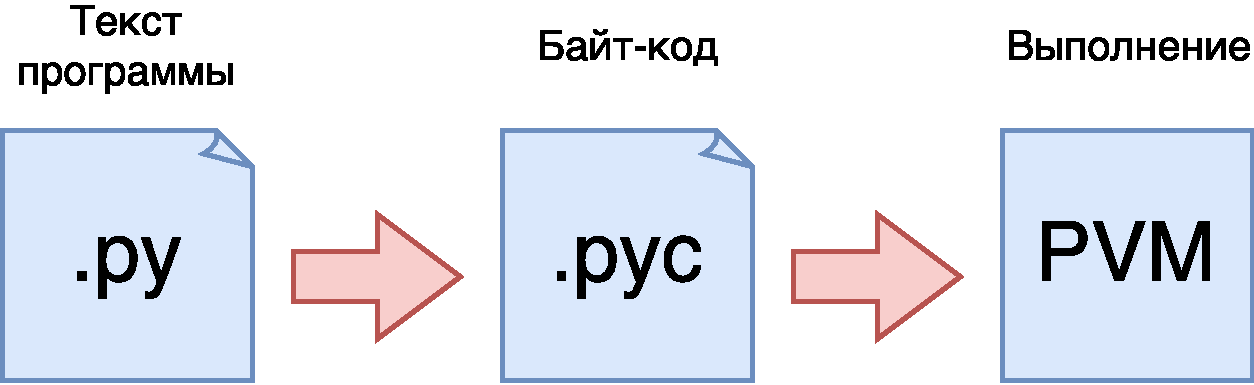
\includegraphics[scale=0.4]{chart.pdf}
\end{figure}

байт-код $\neq$ машинный код $\Rightarrow$ 
\begin{enumerate}
	\item Python медленнее C и C++
	\item Скомпилированная программа платформонезависима
\end{enumerate}
\end{frame}

\begin{frame}{Версии Python}

{Вы можете встретить две несовместимых версии Python}

\hfill

\textbf{Python 2.x:}
\begin{itemize}
\item[--] Официальная разработка и поддержка остановлены 
\item[+] Всё ещё используется в некоторых IT компаний
\end{itemize}

\hfill

\textbf{Python 3.x:}
\begin{itemize}
\item[+] Активно развивается (версия 3.10 выходит в октябре 2021)
\item[+] Исправлены многие ошибочные архитектурные решения Python 2.x

\end{itemize}

\hfill

Задания в систему будут приниматься на Python 3.6. Рекомендуется установить именно эту версию.
\end{frame}

\begin{frame}{Установка Python}

\textbf{Простой и рекомендуемый способ (для всех ОС).}

Скачать дистрибутив \href{https://www.anaconda.com/download/}{Anaconda}, содержащий интерпретатор и предустановленные модули.

\hfill

Для установки новых пакетов рекомендуется использовать систему управления пакетами pip.

\hfill

\textbf{Для продвинутых:} можно создавать отдельные окружения (своя версия языка, свой набор библиотек) под свои нужды (например, для разных учебных курсов).

\end{frame}

\begin{frame}{Работа с интерпретатором в терминале}

Самый простой способ работы --- запуск интерпретатора в терминале (интерактивный режим):

\begin{figure}
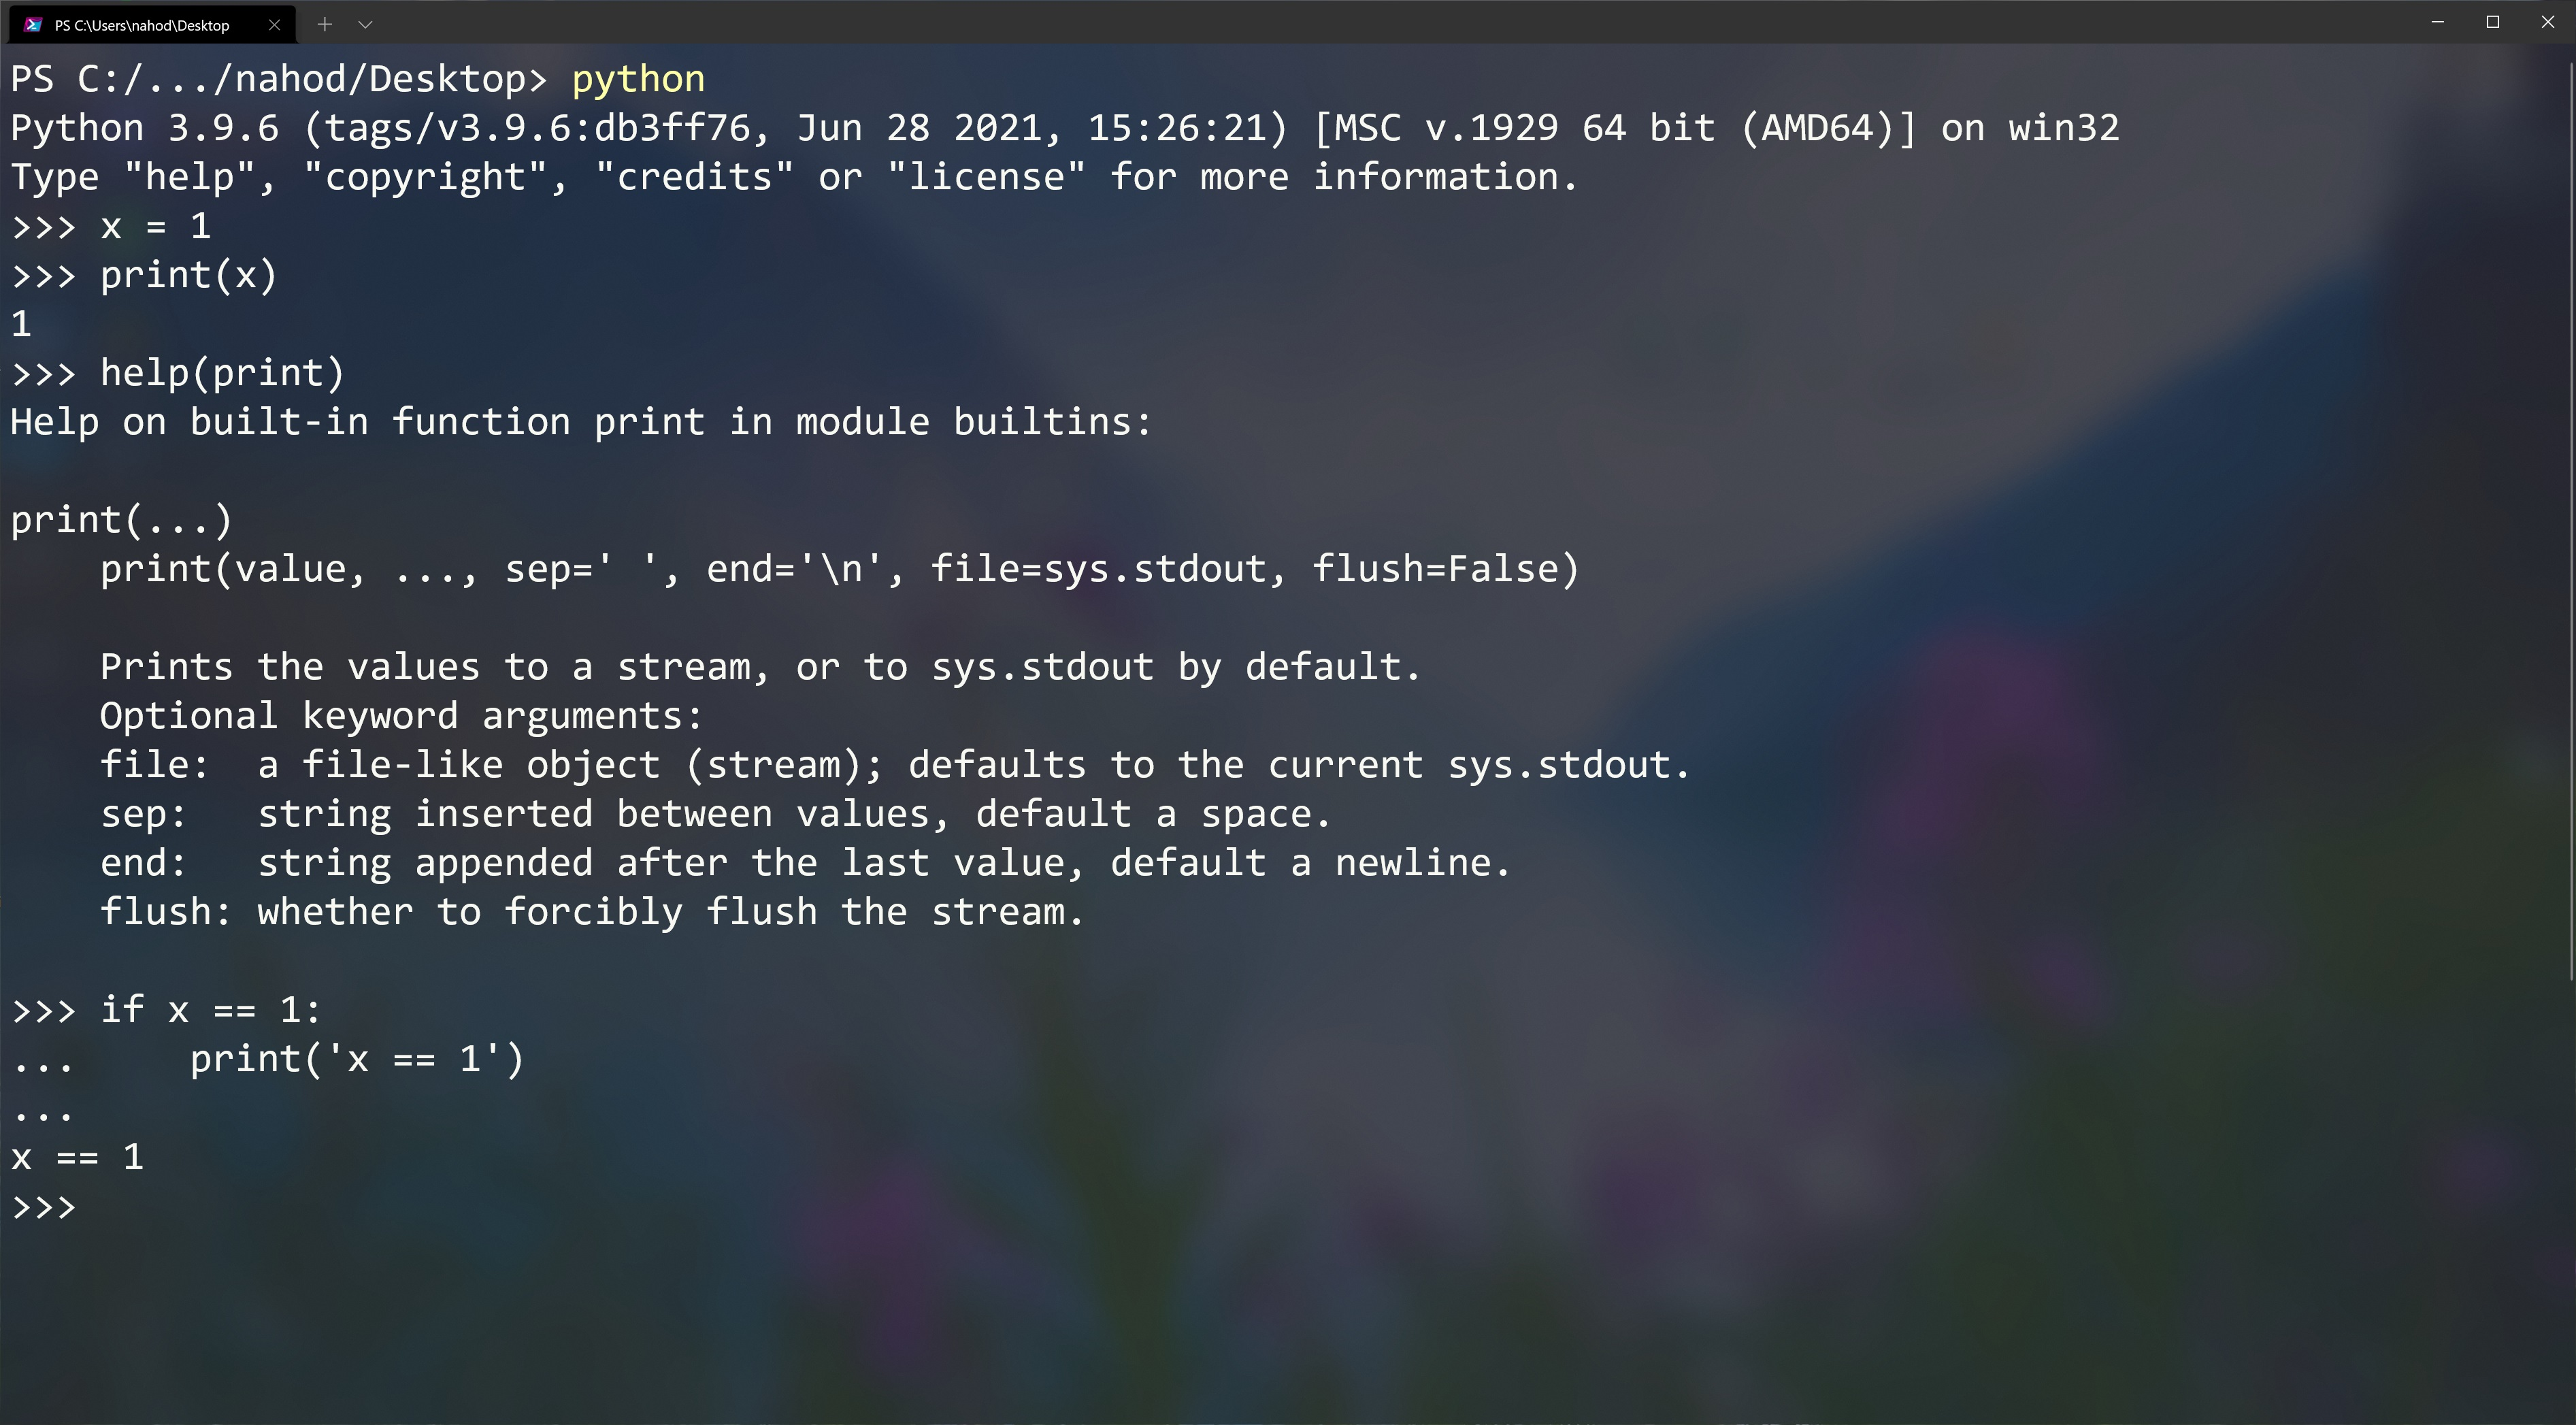
\includegraphics[scale=0.18]{terminal.jpg}
\end{figure}

\end{frame}

\begin{frame}{Интерактивная среда --- Jupyter Notebook}

Интерактивный <<терминал>>, нечто среднее между интерактивном режимом и IDE. Позволяет легко работать с графикой/таблицами/динамическим содержимым, код постоянно сохраняется:

\begin{figure}
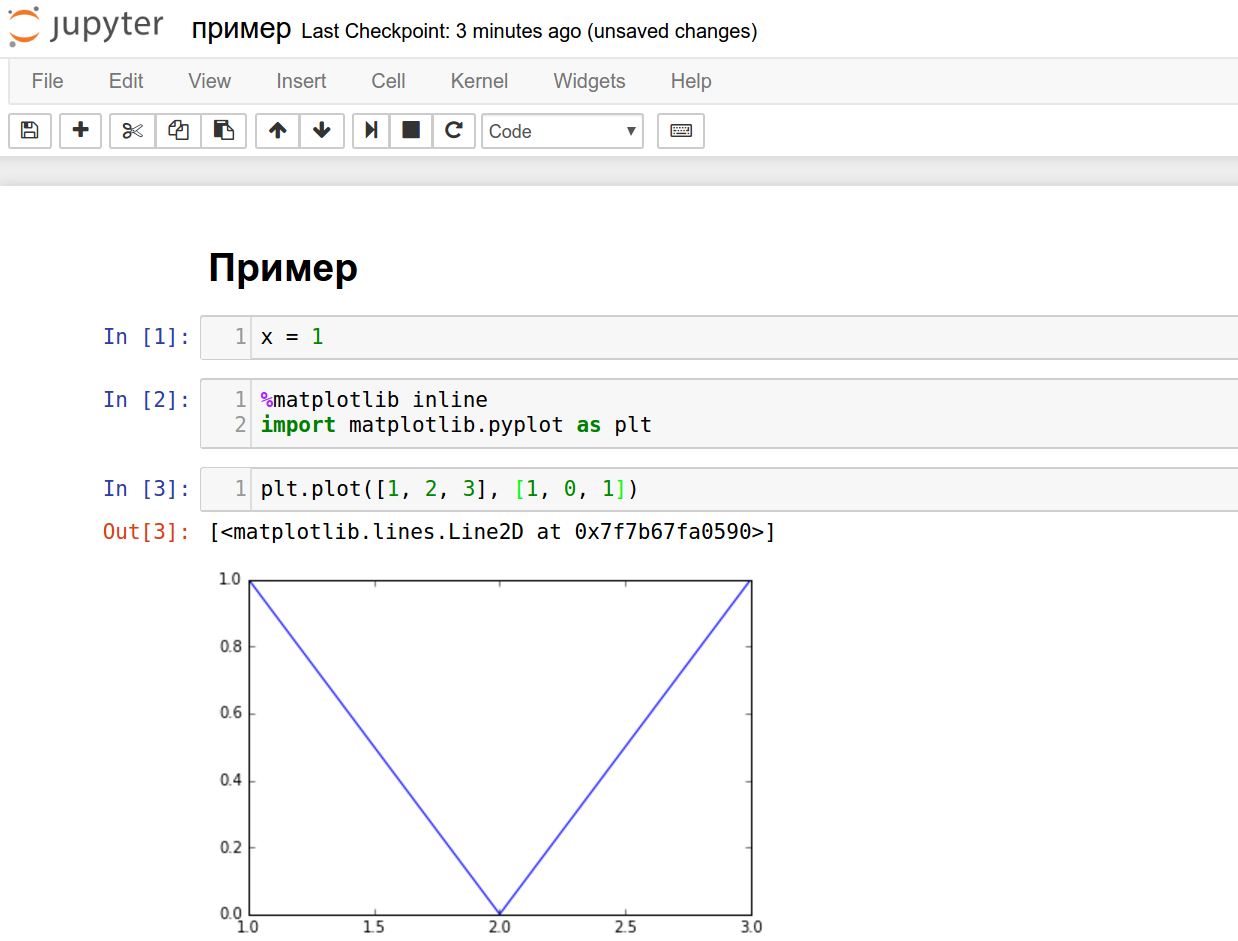
\includegraphics[scale=0.2]{jupyter.png}
\end{figure}

\end{frame}

\begin{frame}{Работа в IDE}

\begin{itemize}
\item PyCharm (свободно доступна Community Edition)
\item VSCode (свободно доступна)
\item Spyder (входит в Anaconda)
\end{itemize}

Много возможностей: отладчик, автоматическая проверка стиля, встроенный терминал.

\begin{figure}
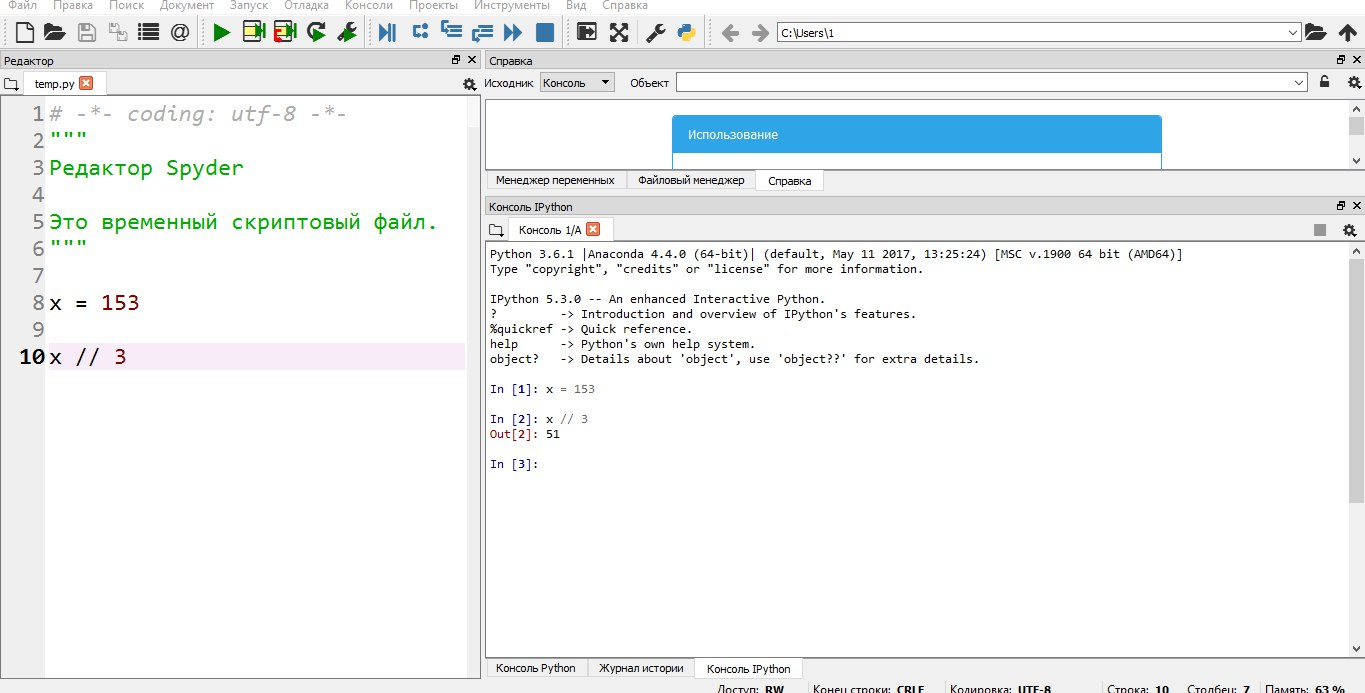
\includegraphics[scale=0.2]{spyder.jpg}
\end{figure}

\end{frame}


\begin{frame}{Список литературы по Python}

Рекомендуется всем начинающим ознакомиться с учебником Лутца до 7 части включительно.

\hfill

\begin{thebibliography}{1}
\item The Python Tutorial

\small{\href{https://docs.python.org/3/tutorial/}{https://docs.python.org/3/tutorial/}}

\item Учебник Python 3.1 

\small{\href{https://ru.wikibooks.org/wiki/Python/\%D0\%A3\%D1\%87\%D0\%B5\%D0\%B1\%D0\%BD\%D0\%B8\%D0\%BA_Python_3.1}{https://ru.wikibooks.org/wiki/Python/Учебник\_Python\_3.1}}


\item Лутц М. --- Изучаем Python (4-e издание и выше)

(легко найти в интернете)

\item Курс CSC <<Программирование на Python>> (видеолекции)

\small{\href{https://compscicenter.ru/courses/python/2015-autumn/classes/}{https://compscicenter.ru/courses/python/2015-autumn/classes/}}

\end{thebibliography}

\end{frame}

\begin{frame}{Список материалов по занятию}
\begin{thebibliography}{1}

\item Стайлгайд языка Python PEP8

\small{\href{https://www.python.org/dev/peps/pep-0008/}{https://www.python.org/dev/peps/pep-0008/}}

\small{\href{https://pythonworld.ru/osnovy/pep-8-rukovodstvo-po-napisaniyu-koda-na-python.html}{https://pythonworld.ru/osnovy/pep-8-rukovodstvo-po-napisaniyu-koda-na-python.html}}

\item Почему существует так много Питонов?

\small{\href{https://habrahabr.ru/post/209812/}{https://habrahabr.ru/post/209812/}}

\item Беглый обзор внутренностей интерпретатора Python

\small{\href{https://www.youtube.com/watch?v=zOuxxnUY4lg}{https://www.youtube.com/watch?v=zOuxxnUY4lg}}

\item Code Like a Pythonista: Idiomatic Python

\small{\href{http://python.net/~goodger/projects/pycon/2007/idiomatic/handout.html}{http://python.net/~goodger/projects/pycon/2007/idiomatic/handout.html}}


\end{thebibliography}


\end{frame}


%
%\begin{frame}[fragile]\frametitle{Пример сложной ситуации}
%Подробно разберём пример программы:
%
%\begin{minted}{python}
%>>> x = 317 
%>>> x = ['m', 'm', 'p']
%>>> y = x
%>>> x[0] = "c"
%>>> x = ['m', 's', 'u']
%>>> print(x)
%['m', 's', 'u']
%>>> print(y)
%['c', 'm', 'p']
%\end{minted}
%
%\textcolor{red}{Как это работает?}
%
%\end{frame}
%
%\begin{frame}[fragile]\frametitle{Создание нового объекта}
%\begin{minted}{python}
%>>> x = 317 
%\end{minted}
%
%Что концептуально происходит:
%\begin{enumerate}
%\item Создается \textit{объект}, представляющий число \mintinline{python}{317} 
%\item Создается \textit{переменная} \mintinline{python}{x}, если она еще отсутствует 
%\item  В переменную \mintinline{python}{x} записывается \textit{ссылка} на созданный объект
%\end{enumerate}
%
%\begin{figure}
%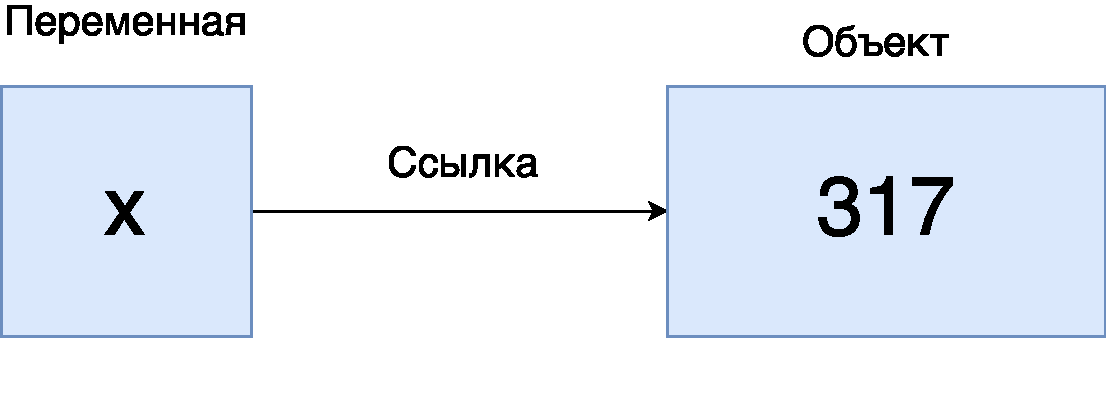
\includegraphics[scale=0.3]{diag1.pdf}
%\end{figure}
%
%\end{frame}
%
%
%\begin{frame}[fragile]\frametitle{Изменение ссылки, уничтожение старого объекта}
%\begin{minted}{python}
%>>> x = ['m', 'm', 'p']
%\end{minted}
%
%\begin{enumerate}
%\setcounter{enumi}{3}
%\item Создается \textit{объект}, представляющий список \mintinline{python}{['m','m','p']}
%\item В переменную \mintinline{python}{x} записывается \textit{ссылка} на новый объект
%\item Объект, представляющий \mintinline{python}{317}, уничтожается
%
%(сборка мусора)
%\end{enumerate}
%
%\begin{figure}
%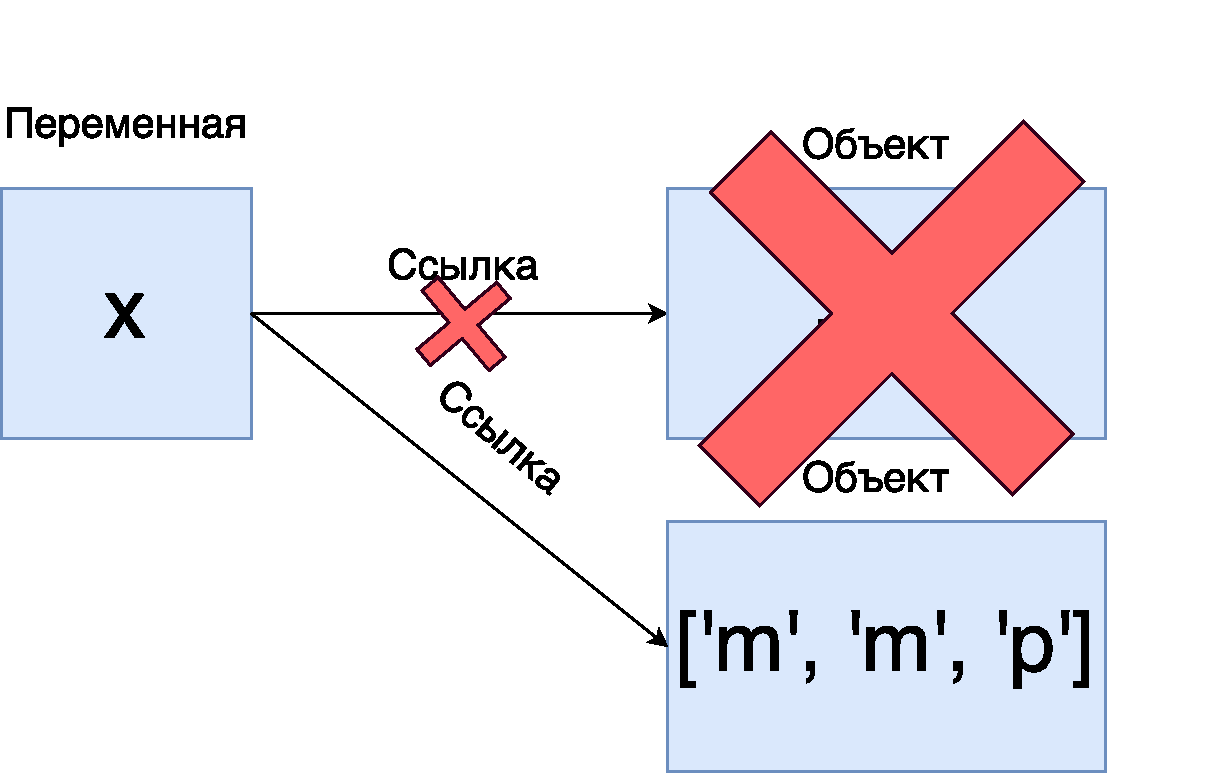
\includegraphics[scale=0.3]{diag2.pdf}
%\end{figure}
%
%\end{frame}
%
%\begin{frame}[fragile]\frametitle{Новая переменная ссылается на старый объект}
%\begin{minted}{python}
%>>> y = x
%\end{minted}
%
%\begin{enumerate}
%\setcounter{enumi}{6}
%\item Создаётся переменная \texttt{y} 
%\item В переменную \mintinline{python}{y} записывается \textit{ссылка} на уже существующий объект
%\end{enumerate}
%\begin{figure}
%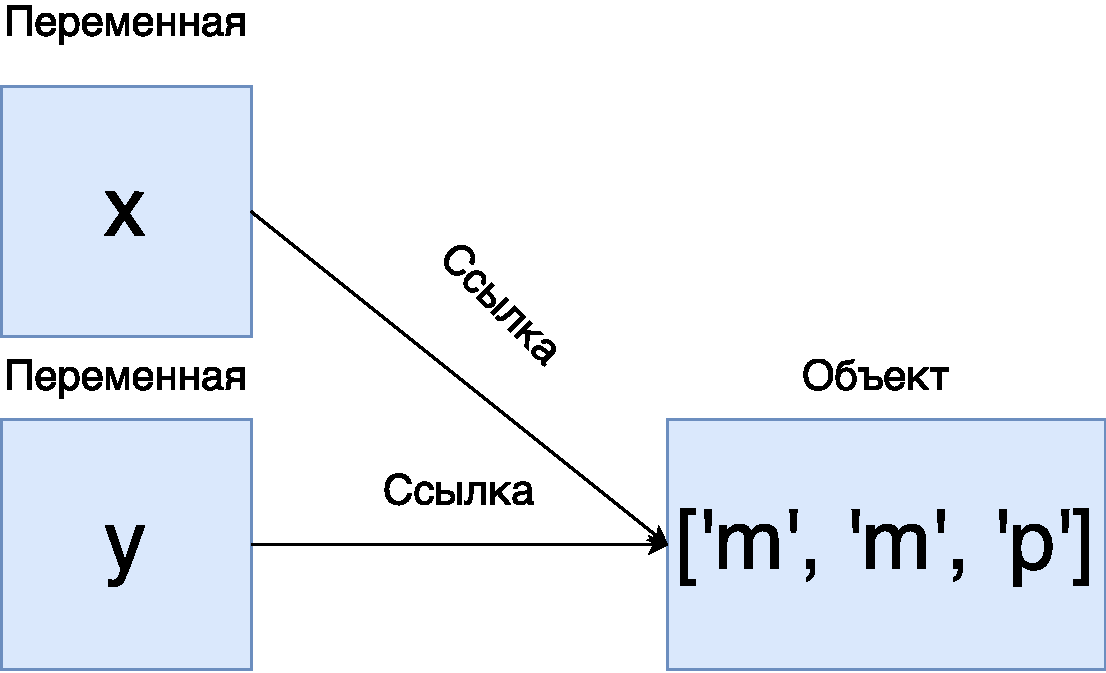
\includegraphics[scale=0.3]{diag3.pdf}
%\end{figure}
%
%\end{frame}
%
%\begin{frame}[fragile]\frametitle{Изменение объекта}
%\begin{minted}{python}
%>>> x[0] = "c"
%\end{minted}
%
%
%\begin{enumerate}
%\setcounter{enumi}{8}
%\item Меняется содержимое объекта с  \mintinline{python}{['m','m','p']} на  \mintinline{python}{['с','m','p']}
%\end{enumerate}
%
%\begin{figure}
%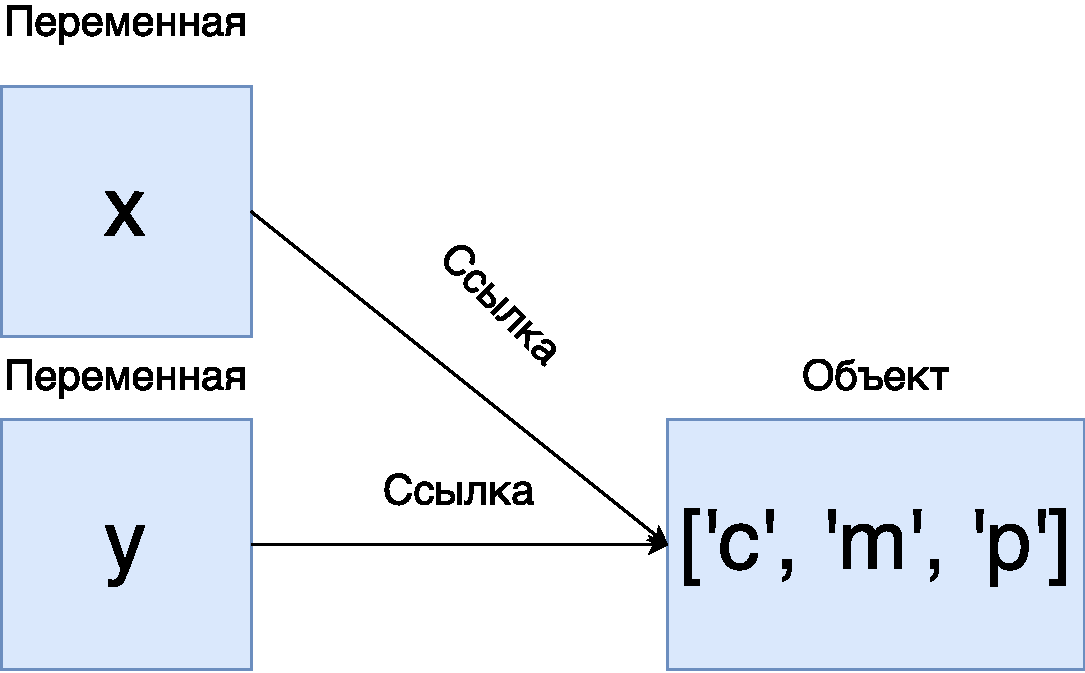
\includegraphics[scale=0.3]{diag4.pdf}
%\end{figure}
%
%
%\end{frame}
%
%\begin{frame}[fragile]\frametitle{Объект не уничтожается, если на него что-то ссылается}
%\begin{minted}{python}
%>>> x = ['m','s','u']
%\end{minted}
%
%\begin{enumerate}
%\setcounter{enumi}{9}
%\item Создаётся объект, соответствующий  \mintinline{python}{['m','s','u']}
%\item В переменную \mintinline{python}{x} записывается \textit{ссылка} на новый объект
%\item Старый объект не удаляется, так как на него ссылается \mintinline{python}{y}
%\end{enumerate}
%
%\begin{figure}
%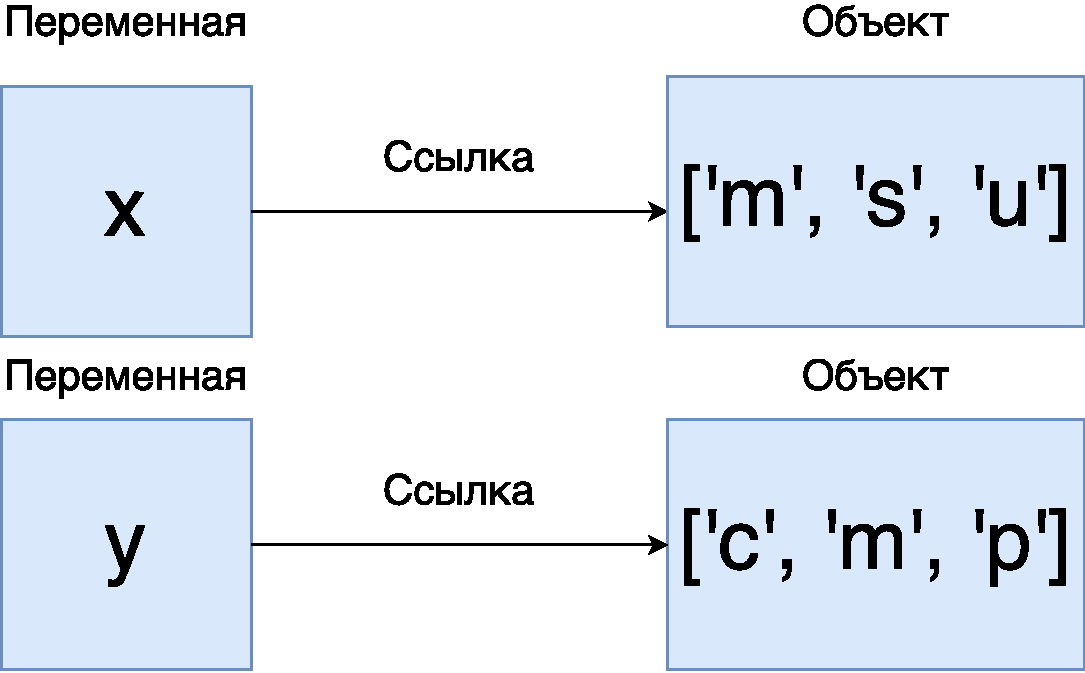
\includegraphics[scale=0.3]{diag5.pdf}
%\end{figure}
%
%\end{frame}
%
%\begin{frame}{Что надо запомнить?}
%\begin{enumerate}
%\item Одной переменной в разное время могут соответствовать объекты разных типов
%\item При присваивании не происходит копирование объекта
%\item Есть некоторые тонкости, о которых мы поговорим позднее
%\end{enumerate}
%\end{frame}
%
%
%\begin{frame}{Список литературы по Python}
%\begin{thebibliography}{1}
%\item The Python Tutorial
%
%\small{\href{https://docs.python.org/3/tutorial/}{https://docs.python.org/3/tutorial/}}
%
%\item Учебник Python 3.1 
%
%\small{\href{https://ru.wikibooks.org/wiki/Python/\%D0\%A3\%D1\%87\%D0\%B5\%D0\%B1\%D0\%BD\%D0\%B8\%D0\%BA_Python_3.1}{https://ru.wikibooks.org/wiki/Python/Учебник\_Python\_3.1}}
%
%
%\item Лутц М. --- Изучаем Python (4-e издание и выше)
%
%(легко найти в интернете)
%
%\item Курс CSC <<Программирование на Python>> (видеолекции)
%
%\small{\href{https://compscicenter.ru/courses/python/2015-autumn/classes/}{https://compscicenter.ru/courses/python/2015-autumn/classes/}}
%
%\end{thebibliography}
%
%\end{frame}
%
%\begin{frame}{Список материалов по занятию}
%\begin{thebibliography}{1}
%\item Почему существует так много Питонов?
%
%\small{\href{https://habrahabr.ru/post/209812/}{https://habrahabr.ru/post/209812/}}
%
%\item Беглый обзор внутренностей интерпретатора Python
%
%\small{\href{https://www.youtube.com/watch?v=zOuxxnUY4lg}{https://www.youtube.com/watch?v=zOuxxnUY4lg}}
%
%\item Code Like a Pythonista: Idiomatic Python
%
%\small{\href{http://python.net/~goodger/projects/pycon/2007/idiomatic/handout.html}{http://python.net/~goodger/projects/pycon/2007/idiomatic/handout.html}}
%
%
%\end{thebibliography}
%
%
%\end{frame}


\end{document}